
\section{Contextualização}\label{sec:contexto}


Para lidar com mudanças e crescentes necessidades de negócios, sistemas de software estão em constante evolução.
Atividades de evolução do softwarafa.re podem abranger desde a manutenção até a substituição total do sistema~\cite{seacord_2003}. 
De acordo com~\citeonline{Lientz_1978} e~\citeonline{Pressman_2009}, a manutenção de software é a atividade mais custosa no ciclo de vida do sistema de software. 
Essa atividade inclui um conjunto de tarefas necessárias para modificar o software existente e ainda deve-se preservar sua integridade.
As tarefas de manutenção de software podem ser vistas como modificações incrementais que adicionam ou atualizam um conjunto de funcionalidades, ou corrigem falhas do projeto.
Usualmente, com o passar do tempo, a integridade conceitual do sistema tende a diminuir, o que afeta a sua qualidade.
%Essa deterioração é conhecida na literatura como o fenômeno de envelhecimento~\cite{Fowler1999}, e lidar com esse fenômeno não é uma atividade trivial e barata.

Uma técnica comum e amplamente utilizada para lidar com tal problema é a reestruturação de software visando melhorar o projeto do software (do inglês - \emph{design}). Uma etapa da reestruturação de software e utilizada no paradigma orientado a objetos é comumente chamada de refatoração~\cite{OPDYKE_1992, Fowler1999, Mens04}. Refatoração foi primeiramente proposta por~\citeonline{OPDYKE_1992} como uma metodologia para reestruturar programas. Seguindo a mesma linha de pensamento, pesquisadores como \citeonline{Fowler1999} tornaram a refatoração uma disciplina comumente conhecida e aplicada, a qual é um processo disciplinado e utilizado para melhorar a estrutura do software, preservando o comportamento do mesmo~\cite{Fowler1999}. Com o apoio ferramental adequado, a refatoração pode ser uma maneira eficiente e eficaz para: (\textit{i}) ajudar a melhorar o projeto do software, (\textit{ii}) tornar o software mais fácil de ser entendido, e (\textit{iii}) auxiliar na identificação de erros. %Na literatura é possível identificar um conjunto de ferramentas, automáticas ou semiautomáticas, que auxiliam na aplicação de refatorações (refs). 


Outra linha de pesquisa é a Engenharia Dirigida por Modelos (do inglês - \sigla{MDE}{\textit{Model-Driven Engineering}}). 
Usualmente, pesquisas encontradas na literatura sobre refatorações estão mais focadas em criar ferramentas e abordagens para refatorações que ocorrem no âmbito do código-fonte. 
No entanto, com o surgimento da MDE e a adoção de muitas ferramentas que permitem gerar código a partir de diagramas, aumentou-se o interesse e a necessidade de ferramentas de apoio a refatorações em nível de modelo. Na verdade, de acordo com~\citeonline{Mens04}, a adaptação de ferramentas de refatoração para fornecer apoio à aplicação de refatorações em modelo pode ser de grande utilidade. Algumas motivações podem ser destacadas para a realização dessas adaptações: (\emph{i}) modelos podem fornecer uma visão abstrata do sistema; assim, visualizações de mudanças estruturais são mais fáceis de serem visualizadas e detectadas; (\emph{ii}) problemas descobertos ainda na fase de projeto podem ser solucionados diretamente no modelo, aumentando a produtividade; (\emph{iii}) a capacidade de explorar caminhos alternativos de decisões é muito mais barato em nível de modelo~\cite{Mens_2006}, uma vez que não se faz necessário a alteração direta do código-fonte, fazendo com que o sistema ainda opere enquanto mudanças são testadas pelo modernizador.


Refatorações em modelos tendem a ser mais complexas do que refatorações aplicadas em código-fonte~\cite{Mens_2006}, uma vez que, além das refatorações, é necessária também a realização de uma atividade para verificar a consistência do modelo e manter a sincronização dele, bem como suas visões~\cite{KolahdouzRahimi20145}. Segundo~\citeonline{Gorp}, desenvolvedores de software utilizam refatorações em nível de projeto e, assim, é intuitivo explorar os conceitos de MDE usando a UML para a aplicação de refatorações~\cite{Salem_2008, Gorp, Egyed_2008, Briand_2006, staron2004implementing}. Nesse sentido, vários pesquisas iniciaram-se com o objetivo de implementar refatorações no contexto da UML~\cite{revisao_sistematica_uml_refactoring}. Uma das vantagens em se utilizar refatorações em nível de modelos, tais como a UML, é que os desenvolvedores de software não precisam se preocupar com características específicas de linguagens de programação (Java, C++, C\#, etc). Além disso, modelos fornecem uma visão abstrata do sistema, assim, o engenheiro de software pode facilmente visualizar e verificar quais refatorações devem ser aplicadas no sistema. 

No entanto, utilizar apenas os diagramas da UML não é uma abordagem adequada para representar todos os artefatos de um sistema de software~\cite{Gorp, KolahdouzRahimi20145, revisao_sistematica_uml_refactoring}. Isso ocorre principalmente porque a UML não consegue representar todas as construções de um determinado sistema. Por exemplo, declarações internas de um método não são consideradas no contexto do metamodelo da UML. Além disso, a UML não contém um conjunto de metaclasses para representar todos os artefatos de um sistema e com ela não é possível representar níveis mais baixos de abstração de um sistema, como o código-fonte, nem mesmo representar níveis mais altos, como a arquitetura do sistema e regras de negócios. Utilizando o metamodelo da UML, poucas informações do código-fonte são representadas, por exemplo, nome da classe, nome do método e seus parâmetros, atributos e tipos.  

Com o objetivo de padronizar o processo de reengenharia o \textit{Object Management Group} (OMG) criou, em 2003, uma força tarefa para analisar e evoluir os tradicionais processos de reengenharia, formalizando-os e fazendo com que eles fossem totalmente apoiados por modelos~\cite{ADM:OMG}. Logo, o termo Modernização Dirigida a Arquitetura (do inglês - \sigla{ADM}{\textit{Architecture-Driven Modernization}}) surgiu como uma solução para os problemas de padronização. A ADM é um processo de modernização de sistemas legados que utiliza um conjunto de metamodelos para representar completamente um sistema por meio de diferentes representações arquiteturais. Esses modelos são, então, submetidos à refatorações, otimizações e, posteriormente, o código-fonte pode ser gerado novamente por meio de atividades de engenharia avante. Durante a modernização de um sistema, são gerados vários modelos de acordo com os metamodelos da ADM, que representam diferentes partes/visões do sistema, como: fluxo de dados, banco de dados, elementos de programação (métodos, classes, tipos de dados, etc.) e arquitetura~\cite{PerezCastillo20121370}.

O Knowledge Discovery Metamodel (KDM) é o principal metamodelo da ADM com uma ampla quantidade de metaclasses para representar desde os níveis mais baixos de abstração de um sistema (código-fonte), até níveis mais altos (arquitetura do sistema), permitindo a representação de conceitos de qualquer domínio~\cite{KDM:specification,KDM:ISO}. Diferentemente de metamodelos existentes, o KDM mantém todas as visões/representações do sistema em uma única instância; o KDM pode ser considerado como uma família de metamodelos, uma vez que compartilha a consistência e terminologia homogênea. 

A ideia principal da ADM é que a comunidade comece a desenvolver ferramentas que atuem apenas sobre instâncias do metamodelo KDM, ao invés de serem dependentes de plataformas e linguagens específicas. Por exemplo, um catálogo de refatorações~\cite{durelli_catalogo} para o KDM tem o poder de reestruturar um sistema independentemente da linguagem de programação que foi usada em seu desenvolvimento, já que as refatorações ocorrem nos modelos. Outro exemplo seria a aplicação de técnicas de mineração de interesses transversais, utilizando como base o metamodelo KDM~\cite{Durelli:2013_ACM, dani_san, daniel_san_journal}.


No entanto, embora a ADM tenha investido esforços objetivando fornecer metamodelos para auxiliar o engenheiro de modernização a conduzir a reengenharia de um sistema, seguindo todas as diretrizes de MDE, a ADM ainda não fornece instruções de como criar, reusar e/ou aplicar refatorações no metamodelo KDM, nem mesmo como manter uma determinada instância do KDM sincronizada após a aplicação de refatorações. Assim, tais particularidades devem ser tratadas pelos engenheiros de modernização. Isso faz com que os engenheiros criem suas próprias soluções. Porém, usualmente, tais soluções são proprietárias e específicas, o que pode dificultar a interoperabilidade entre diferentes soluções. Dessa forma, nesta tese é apresentada uma abordagem para criação e disponibilização de refatorações para o metamodelo KDM, bem como um apoio ferramental que permite aplicá-las em diagramas de classe da UML. 

%Esta tese de doutorado aborda as seguintes questões de pesquisas (QP):

%\begin{itemize}
% 	\item \textbf{QP$_1$}: Qual é o estado da arte de refatorações no contexto da ADM, e principalmente para o metamodelo KDM?;
% 	\item \textbf{QP$_2$}: Como manter todas as visões do metamodelo KDM sincronizado após a aplicação de um conjunto de refatorações?;
 %	\item \textbf{QP$_3$}: Como especificar refatorações para que elas possam ser disponibilizadas/reutilizadas de forma independente de linguagem e plataforma de programação?;
 %	\item \textbf{QP$_4$}: Como automatizar o processo de aplicação de refatorações dentro do contexto da ADM e KDM?.
 %\end{itemize} 


\section{Motivações}\label{sec:justificativa_e_motivacao}

%Refatorações são técnicas utilizadas para melhorar a estrutura do software~\cite{Fowler1999}. Hoje em dia é evidente que a refatoração é de suma importância para melhorar a qualidade do código-fonte. Embora a refatoração para modelos tenha alcançado bastante reconhecimento e aceitação~\cite{Salem_2008, Gorp, Egyed_2008, Briand_2006, staron2004implementing}, ainda se faz necessárias pesquisas nessa área~\cite{revisao_sistematica_uml_refactoring, durelli_systematic_mapping}. 

%Embora a ADM e o KDM tenham sido propostos para auxiliar todo o processo da modernização de sistemas por meio de modelos, ainda hoje existe uma ausência de abordagens e apoios computacionais para auxiliar os engenheiros de modernização durante a aplicação de refatorações de forma consistente em instâncias do metamodelo KDM\footnote{É importante ressaltar que para facilitar a leitura e o entendimento  desta Tese em vários pontos o termo \aspas{refatorações para o KDM} será utilizada de forma intercambiável a \aspas{refatorações aplicadas em instâncias do metamodelo KDM}.}. Dessa forma, usualmente os engenheiros de modernização precisam desenvolver suas próprias abordagens e apoios ferramentais para refatorar diversos sistemas. Tais soluções tendem a ser proprietárias e consequentemente tornam-se difíceis de serem reutilizadas e dificulta a interoperabilidade entre outras ferramentas. Assim, é possível concluir que este é um campo atual e promissor para novas pesquisas. Nesse contexto, a pesquisa apresentada nesta tese visa a contribuir para a criação de abordagens e apoios computacionais para auxiliar os engenheiros de software durante a aplicação de refatorações para o KDM. No contexto desta Tese, as principais motivações são:

As motivações que levaram ao desenvolvimento desta tese foram:

\begin{enumerate}

\item Carência de ferramentas de modernização que permitem aplicar refatorações em diagramas UML que são representações gráficas de modelos KDM. Isto é, a maioria das ferramentas que permitem refatorações em diagramas UML, mantém internamente apenas o metamodelo UML. Isso faz com que os algoritmos de refatoração não sigam o padrão KDM, impedindo seu reúso em ferramentas de modernização que utilizam esse padrão. Além disso, o metamodelo UML restringe bastante o número de refatorações possíveis em processos de modernização.


\item Escassez de abordagens para criar refatorações para o KDM. Esta motivação está relacionada com a ausência de diretrizes claras que guiem o engenheiro de modernização na criação de refatorações para o metamodelo KDM. A ausência de diretrizes desse tipo faz com que os engenheiros de modernização sigam procedimento \textit{ad-hoc} que podem levar a refatorações de baixa qualidade;


%buscar quais são as diretrizes que permitem o engenheiro de modernização criar refatorações tradicionais para o metamodelo KDM. A ausência de diretrizes desse tipo dificulta a criação de refatorações para o KDM, fazendo com que engenheiros de modernização tenham que criar suas próprias soluções;

%\item Escassez de abordagens para criar refatorações para o KDM; buscar quais são as diretrizes que permitem o engenheiro de modernização criar refatorações tradicionais para o metamodelo KDM. A ausência de diretrizes desse tipo dificulta a criação de refatorações para o KDM, fazendo com que engenheiros de modernização tenham que criar suas próprias soluções;


%O SRM objetiva definir uma terminologia comum para a especificação de refatorações para facilitar o reúso e a interoperabilidade entre ferramentas. Esse objetivo é apoiado por um conjunto de metaclasses que definem meta-atributos específicos para representar informações (metadados) de uma refatoração, auxiliando o compartilhamento das refatorações de forma intuitiva para os modernizadores.

\item Ausência de uma terminologia comum para a especificação de refatorações. Essa ausência dificulta o reúso e a interoperabilidade entre ferramentas de modernização. Refatorações são atividades menores dentro de processos de modernização. Assim, a criação de um metamodelo separado, flexibiliza a especificação de refatorações e permite que elas sejam reusadas dentro de transformações maiores. %Esse metamodelo deve definir metaclasses e meta-atributos específicos para representar informações (metadados) de uma refatoração, aumentando o reúso e a interoperabilidade das refatorações. 


%A grande maioria desses cenários geralmente necessita e é precedida por refatorações de granularidade fina. Dessa forma, pode-se dizer que refatorações são atividades menores dentro de processos de modernização. Um metamodelo separado para refatorações flexibiliza a especificação de refatorações e permite que elas sejam reusadas dentro de transformações maiores.


%Ausência de uma infraestrutura de suporte ao reúso de refatorações para o KDM. A ausência de uma infraestrutura desse tipo faz com que engenheiros de modernização criem suas próprias soluções para especificar, armazenar e disponibilizar refatorações, dificultando o reúso das refatorações em outros contextos; 



%\item Ausência de um metamodelo que reúna as principais informações relacionadas com refatorações. Refatorações são disponibilizadas por meio de linguagem natural~\cite{Fowler1999}, porém não são facilmente reutilizadas. Uma abordagem promissora é lidar com a refatoração de forma independente da linguagem – aumentando assim as possibilidades de reutilização das refatorações;

%\item Embora a ADM forneça um conjunto de metamodelos para auxiliar o engenheiro de modernização a conduzir modernização até esse momento a ADM não provê instruções para auxiliar o engenheiro a promover o reúso de refatorações juntamente com os seus metamodelos padronizados (por exemplo, KDM) durante o processo de modernização. Essa limitação faz com que o engenheiro de modernização crie suas próprias soluções/refatorações, resultando em um possível atraso no processo de modernização. Contudo, as soluções/refatorações  definidas não são facilmente reutilizadas, pois tendem a ser proprietárias e específicas de linguagem e plataforma. Uma solução promissora é lidar com a refatoração de forma independente da linguagem – aumentando assim as possibilidades de reutilização de refatorações. Dessa forma, existe a motivação de criar uma metamodelo para auxiliar o engenheiro de modernização a promover o reúso de refatorações no contexto da ADM e principalmente de forma integrada com o metamodelo KDM. 




%\item Carência de apoios computacionais efetivos para auxiliar o engenheiro de software durante a aplicação, disponibilização e reúso de refatorações para o KDM. A escassez de apoio computacional efetivo pode também dificultar a condução adequada de refatorações para o KDM.

\end{enumerate}

Nesse contexto, a pesquisa aqui apresentada visa contribuir para a definição de uma abordagem que almeja a criação, a disponibilização e a aplicação de refatorações para o KDM.


%É comumente observado que a atividade de refatoração é pertinente a qualquer processo de modernização. Dessa forma, quando um sistema é representado utilizando diferentes visões conceituais para representar níveis de abstração do sistema (por exemplo, visão arquitetural, visão de código-fonte, visão do banco de dados, etc), um acidente comum que surge durante atividades de refatorações é a dessincronização das instâncias do metamodelo, resultando em visões inconsistente após a aplicação de uma refatoração. Dessa forma, no contexto do metamodelo KDM existe uma carência em abordagens e ferramentas que auxiliam a sincronizar tais mudanças após a aplicação de um conjunto de refatorações no KDM. Pesquisas recentes sugerem que a aplicação de técnicas de propagação de mudanças podem auxiliar na identificação e atualização de todas as instâncias/visões do KDM, permitindo assim manter todas as visões/instâncias do metamodelo KDM sincronizadas [7]–[10]. 
%Usualmente, o processo de refatorações em modelos é mais complexo do que refatoções em código-fonte (ref), uma vez que além das refatorações é necessário também a realização de atividades para verificar a consistência do modelo, manter a sincronição do modelo e suas visões, etc. Em consequência disso, poucos avanços significativos foram conseguidos em relação a definição de refatoração para o metamodelo KDM.
%
%Pode-se destacar as principais motivações para aplicar refatorações em nível de modelos, principalmente utilizando o KDM:

%\begin{itemize}

    %\item Embora a refatoração para modelos tenha alcançado bastante reconhecimento e aceitação, até o presente momento apenas trabalhos desenvolvido no contexto do metamodelo \sigla{UML}{\textit{Unified Modeling Language}} foram encontrados e consolidados na literatura~\cite{revisao_sistematica_uml_refactoring, durelli_systematic_mapping}. 
    
 %   \item Ausência de abordagens para adaptar e especificar refatorações para o KDM. %Até o presente momento apenas trabalhos desenvolvidos no contexto metamodelo \sigla{UML}{\textit{Unified Modeling Language}} foram encontrados e consolidados na literatura~\cite{revisao_sistematica_uml_refactoring, durelli_systematic_mapping}. Neste contexto, existe uma motivação para criar diretrizes de como adaptar refatorações para o KDM.
    
    %Dessa forma, existe uma ausência de abordagens para o metamodelo KDM, uma vez que o mesmo é um metamodelo mais novo quando comparado a UML. A refatoração de um sistema em geral tende a ser uma atividade complexa; modificações manuais, sem qualquer catálogo de refatoração, bem como um ambiente integrado, pode resultar em efeitos colaterais indesejados e acarretar em um processo tedioso. Neste contexto, existe uma necessidade para elaborar/adaptar um catálogo de refatoração para o metamodelo KDM e também criar um ambiente que auxilie a aplicação de refatorações diretamente no KDM, assim, os engenheiros podem reduzir o tempo e esforço durante a refatoração de sistemas legados e ainda respeitando a interoperabilidade fornecida pelo metamodelo KDM.

%	\item Carência de abordagens e apoios computacionais para manter o metamodelo KDM consistente e sincronizado após a aplicação de refatorações;
	
	%O KDM é um metamodelo que possui um conjunto de metaclasses complementares para representar diferentes artefatos e visões conceituais de um mesmo sistema. Dessa forma, quando refatorações são aplicadas em uma visão conceitual todas as outras visões conceituais do sistema deveriam manter-se consistentes e sincronizadas. No contexto da ADM, e principalmente do metamodelo KDM existe uma carência de abordagens que sincronizam tais refatorações. A aplicação de técnicas de propagação de mudanças podem auxiliar na identificação e atualização de todas as instâncias/visões do KDM, permitindo assim manter todas as visões/instâncias do metamodelo KDM sincronizadas.  

	%Existe um relacionamento complementar entre todas as visões conceituais do metamodelo KDM. Dessa forma, quando refatorações são aplicadas em uma visão conceitual, por exemplo, em uma instância do KDM que representa o código-fonte do sistema, e não é sem considerar a sincronização e consistência de outras visões 
	%\item Embora a refatoração para modelos tenha alcançado bastante reconhecimento e aceitação, até o presente momento apenas trabalhos desenvolvido no contexto do metamodelo \sigla{UML}{\textit{Unified Modeling Language}} foram encontrados e consolidados na literatura~\cite{revisao_sistematica_uml_refactoring, durelli_systematic_mapping}. Dessa forma, existe uma ausência de abordagens para o metamodelo KDM, uma vez que o mesmo é um metamodelo mais novo quando comparado a UML. A refatoração de um sistema em geral tende a ser uma atividade complexa; modificações manuais, sem qualquer catálogo de refatoração, bem como um ambiente integrado, pode resultar em efeitos colaterais indesejados e acarretar em um processo tedioso. Neste contexto, existe uma necessidade para elaborar/adaptar um catálogo de refatoração para o metamodelo KDM e também criar um ambiente que auxilie a aplicação de refatorações diretamente no KDM, assim, os engenheiros podem reduzir o tempo e esforço durante a refatoração de sistemas legados e ainda respeitando a interoperabilidade fornecida pelo metamodelo KDM.


    %\item Na literatura é possível identificar um conjunto de refatorações já validadas e que são usualmente aplicadas em código-fonte, por exemplo, \textit{Extract Class}, \textit{Move Method}, \textit{Move Attribute}, etc. Essas são apenas alguns exemplos de refatorações úteis que não são facilmente reutilizadas na prática durante a condução de modernização de um determinado sistema (fowler, ADM refactoring). Essa limitação pode ser atribuída devido a ausência de um meio padronizado de disponibilizar refatorações. Embora a ADM forneça um conjunto de metamodelos para auxiliar o engenheiro de software a conduzir MDRE até esse momento a ADM não provê instruções para auxiliar o engenheiro a promover o reúso de refatorações juntamente com os seus metamodelos padronizados (por exemplo, KDM) durante o processo de modernização. Essa limitação faz com que o engenheiro crie suas próprias soluções/refatorações, resultando em um possível atraso no processo de modernização. Contudo, as soluções/refatorações  definidas não são facilmente reutilizadas pois tendem a ser proprietárias. Uma abordagem promissora é lidar com a refatoração de forma independente da linguagem – aumentando assim as possibilidades de reutilização de refatorações. Dessa forna, existe uma necessidade de criar uma metamodelo para auxiliar o engenheiro de modernização a promover o reúso de refatorações no contexto da ADM e principalmente de forma integrada com o metamodelo KDM. 
    
    %\item Escassez de meios para disponibilizar e promover o reúso de refatorações no contexto da ADM e KDM. 

%	\item Refatorações são metodologias bem consolidadas e amplamente utilizadas tanto academicamente quanto industrialmente. Usualmente, refatorações são compartilhas e distribuídas por meio de catálogos escritos em linguagem natural.
	%Na literatura é possível identificar um conjunto de refatorações já validadas e que são usualmente aplicadas em código-fonte. 
%	No entanto, refatorações não são facilmente reutilizadas na prática. Essa limitação pode ser atribuída devido a ausência de um meio padronizado de disponibilizar refatorações. Embora a ADM forneça um conjunto de metamodelos para representar diversos artefatos de sistemas de software até esse momento a ADM não provê instruções para auxiliar de como prover o reúso de refatorações. Uma abordagem promissora é lidar com a refatoração de forma independente da linguagem – aumentando assim as possibilidades de reutilização de refatorações. Dessa forna, existe uma necessidade de criar um metamodelo para auxiliar o engenheiro de modernização a promover o reúso de refatorações no contexto da ADM e principalmente de forma integrada com o metamodelo KDM. 

%\end{itemize}


\section{Síntese da Pesquisa Conduzida}\label{sec:introducao:a_abordagem_desenvolvida}

Com base nas motivações apresentadas o trabalho desenvolvido aqui visa auxiliar dois principais atores: (\textit{i}) o engenheiro de modernização\footnote{No contexto desta tese, engenheiro de modernização é aquele que utiliza a abordagem aqui proposta para criar, disponibilizar e reutilizar refatorações para o KDM.} e  (\textit{ii}) o engenheiro de software\footnote{No contexto desta tese, engenheiro de software é aquele que interage com o apoio computacional desenvolvido aqui para aplicar refatorações em instâncias do KDM.}. O engenheiro de modernização é aquele que cria e disponibiliza refatorações para o metamodelo KDM no sentido de facilitar o reúso das mesmas. Por sua vez, o engenheiro de software é aquele responsável por conduzir um processo de modernização e que se utiliza de apoios computacionais para aplicar refatorações existentes.


%pode aplicar refatorações por meio de um apoio computacional.%utilizando o diagrama de classe da UML e de forma transparente um apoio computacional aplica as refatorações em um instância do metamodelo KDM. 



Na Figura~\ref{fig:abordagem_kdm_tese_processo}, uma visão geral do trabalho/pesquisa desenvolvida é apresentada. Note que, a figura é dividida em dois retângulos tracejados. O primeiro retângulo representa os passos da abordagem e o segundo ilustra a condução de um processo de modernização. A abordagem desenvolvida contém dois passos e o processo de modernização é abstraído em apenas um passo. Note também que a figura ilustra o papel do engenheiro de modernização e do engenheiro de software. 
Os dois passos da abordagem são executados pelo engenheiro de modernização e o processo de modernização é executado pelo engenheiro de software. A seguir, uma descrição resumida é apresentada.

O passo \ding{182} consiste na criação de refatorações para o metamodelo KDM. Esse passo é apoiado por seis diretrizes, as quais o engenheiro de modernização segue para criar refatorações para o metamodelo KDM. As refatorações são um conjunto de regras ATL, as quais são criadas por meio da combinação de um conjunto de artefatos: (\textit{i}) mapeamento entre KDM e POO, (\textit{ii}) operações atômicas, (\textit{iii}) \textit{templates}, (\textit{iv}) linguagem de transformação e (\textit{v}) linguagem de restrição.


% A primeira diretriz consiste em identificar os elementos estruturais entre o paradigma orientado a objeto e o metamodelo KDM. Em seguida, o engenheiro de modernização escolhe qual refatoração almeja criar para o KDM. Então, a refatoração é implementada por meio da linguagem de transformação ATL. As restrições (pré- e pós-condições) da refatoração são implementadas em OCL e o engenheiro de modernização pode documentar a refatoração por meio de duas especificações: informal e formal.


%A criação de refatorações para o KDM é apoiada por cinco diretrizesO objetivo é criar diretrizes para que outros engenheiros de modernização possam criar refatorações para o KDM.

%O metamodelo KDM consiste em um conjunto de pacotes para representar diversos artefatos existentes de um sistema de software. Assim, após a aplicação de refatorações é de suma importância manter todos os pacotes/artefatos sincronizados e consistentes. Dessa forma, no passo \ding{183} regras de propagações são realizadas em instância do metamodelo KDM para manter todos os artefatos sincronizados e consistentes de acordo com a refatoração aplicada. 
%O passo \ding{183} consiste na disponibilização de refatorações por meio de um metamodelo aqui definido. Esse metamodelo contém metaclasses que permitem armazenar informações relacionadas com refatorações, desde seu nome até seu mecanismo. O objetivo é permitir e aumentar a interoperabilidade de refatorações para um amplo domínio e auxiliar o engenheiro de modernização a definir refatorações representativas em forma de metadados. Posteriormente as instâncias desse metamodelo são enviadas para um repositório e são reutilizadas por engenheiros de software por meio de um apoio computacional. O apoio computacional \ding{184} também foi definido para auxiliar o engenheiro de software a aplicar refatorações em sistemas representados pelo KDM. Após a aplicação de refatorações é de suma importância manter todos os pacotes/artefatos sincronizados e consistentes. Dessa forma, esse apoio computacional contém um plug-in responsável por implementar regras de propagações que são realizadas em instância do metamodelo KDM. Essas regras mantêm todos os artefatos sincronizados e consistentes de acordo com a refatoração aplicada. 

\begin{figure}[h]
	\centering
	% Requires \usepackage{graphicx}
	\caption{Visão geral da abordagem proposta.}
	\label{fig:abordagem_kdm_tese_processo}
	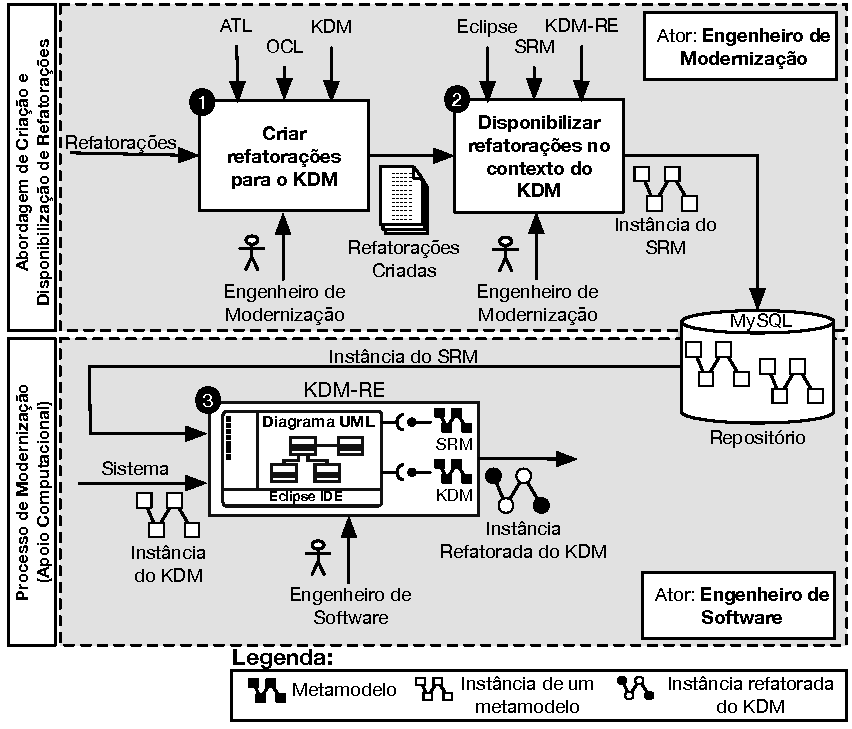
\includegraphics[scale=0.8]{images/NovaFiguraSintexeAbordagem}
	\fautor
\end{figure}

O passo \ding{183} consiste na disponibilização das refatorações criadas por meio de um metamodelo aqui definido, o qual contém metaclasses que permitem armazenar metadados relacionados com refatorações, tais como: o nome da refatoração, sua motivação, autor, pré- e pós-condições e seu mecanismo. O objetivo desse metamodelo é viabilizar o reúso das refatorações dentro de ferramentas de modernização, propiciando a interoperabilidade entre as mesmas. A instanciação desse metamodelo é apoiada por um apoio computacional criado no contexto desta tese denominado KDM-RE, que fornece uma linguagem específica de domínio para auxiliar o engenheiro de modernização durante a instanciação desse metamodelo. Em seguida, as instâncias desse metamodelo são enviadas pelo KDM-RE para um repositório e podem ser reutilizadas por engenheiros de software. 

%É importante salientar que tanto as restrições (pré- e pós-condições) e os mecanismo das refatorações são disponibilizados no metamodelo por meio de linguagens de transformação (ATL) e restrições (OCL). 

O processo de modernização (ver Figura~\ref{fig:abordagem_kdm_tese_processo} \ding{184}) dá enfoque na aplicação de refatorações e a propagação de mudanças por meio do KDM-RE. KDM-RE foi implementado para automatizar a atividade de aplicação e reutilização de refatorações em sistemas representados pelo KDM. As refatorações podem ser aplicadas diretamente em diagramas de classes UML, porém, a refatoração é de fato realizada transparentemente no metamodelo KDM e, posteriormente, replicada nos diagramas de classes UML. Adicionalmente, após a aplicação de refatorações em sistemas representados pelo KDM, é importante manter todos os pacotes/artefatos sincronizados e consistentes. Dessa forma, o KDM-RE também contém um \textit{plug-in} responsável por aplicar regras de propagações, que são realizadas em instância do metamodelo KDM. O intuito desse \textit{plug-in} é manter todos os artefatos sincronizados e consistentes de acordo com a refatoração aplicada.


\section{Objetivos}\label{sec:objetivos}

%A tese subjacente a este trabalho baseia-se no fato de que é possível e benéfico o uso de refatorações para o contexto da ADM, principalmente para o KDM. Nesse contexto, 

O objetivo nesta tese é apresentar uma abordagem para criação e disponibilização de refatorações para o metamodelo KDM, bem como um apoio ferramental que permite aplicá-las em diagramas de classe da UML (ver Figura~\ref{fig:abordagem_kdm_tese_processo}). Mais especificamente, os seguintes objetivos podem ser especificados:%Para que esse objetivo seja alcançado, os seguintes objetivos específicos devem ser atingidos:

\begin{itemize}

    \item Tornar a criação de refatorações para o metamodelo KDM um processo sistemático e guiado, facilitando a tarefa do engenheiro de modernização e procurando garantir que as refatorações desenvolvidas estejam estruturadas corretamente com base nas metaclasses do KDM;
    
    \item %Propor um metamodelo inicial como uma solução para promover o reúso e a interoperabilidade de refatoração. 
    Potencializar o reúso das refatorações desenvolvidas. Este objetivo é apoiado por um metamodelo para a especificação das refatorações. A ideia é que ferramentas de modernização adotem esse metamodelo como base para suas refatorações, permitindo assim o reúso de instâncias de refatorações entre ferramentas. Esse metamodelo possui um conjunto de metaclasses que define meta-atributos específicos para representar informações (metadados) de refatoração, auxiliando, assim, o compartilhamento das refatorações de forma intuitiva entre os engenheiros. %Além disso, esse metamodelo também possui metaclasses e meta-atributos que representam os mecanismos das refatorações, bem como suas pré- e pós-condições;
    
    %\item Viabilizar a disponibilização de refatorações para o metamodelo KDM de forma que possam ser mais facilmente especificadas, disponibilizadas e reusadas; 
    
    %\item Disseminar conhecimentos teórico e técnico que facilitem o reúso e a aplicação de refatorações para o metamodelo KDM em ambientes de modelagem UML;
    

	%\item Definir diretrizes para criar refatorações para o metamodelo KDM;
	
	%\item Especificar e criar um metamodelo para auxiliar engenheiros de modernização a compartilhar, criar e reutilizar refatorações no contexto da ADM e KDM;
	
	%\item Elaborar uma linguagem específica de domínio (do inglês - \sigla{DSL}{\textit{Domain-Specific Language}}). Essa DSL possui duas finalidades, a saber: (\textit{i}) auxiliar o engenheiro de modernização a instanciar o metamodelo de refatoração proposto e (\textit{ii}) facilitar a criação de um conjunto de refatorações de forma guiada e automática;
	
	%\item Criar um repositório totalmente integrado com o apoio ferramental para facilitar o compartilhamento e o reúso de refatorações que estão em conformidade com o metamodelo de refatoração proposto; e
	
	%\item Elaborar regras pré-definidas para manter o metamodelo KDM consistente e sincronizado após a aplicar um conjunto de refatorações;
	
    \item Desenvolver um apoio ferramental totalmente integrado no ambiente de desenvolvimento Eclipse para apoiar a abordagem proposta nesta tese.

\end{itemize}




%A tese subjacente a este trabalho é de que é possível e benéfico o uso de refatorações para o contexto da ADM, principalmente para o KDM. %Além disso, pretende-se viabilizar a reutilização e padronizações de refatorações por meio da utilização de um metamodelo de refatorações. Adicionalmente, planeja-se verificar a possibilidade de manter todas as visões do metamodelo KDM sincronizada e consistentes após a aplicação de um conjunto de refatorações. %e de técnicas de propagação de mudanças para manter todas as visões do KDM sincronizadas e consistentes após a aplicação de uma refatoração. 
%Neste contexto, esta tese de doutorado cobre os seguintes aspectos: 


%\begin{itemize}
%	\item Definir diretrizes para criar refatorações para o metamodelo KDM;
	
%	\item Criar regras pré-definidas para manter o metamodelo KDM consistente e sincronizado após a aplicar um conjunto de refatorações;
	
%	\item Especificar e criar um metamodelo para auxiliar engenheiros de modernização a compartilhar, criar e reutilizar refatorações no contexto da ADM e KDM;
	%\item a elaboração de uma linguagem específica de domínio (do inglês - \sigla{DSL}{\textit{Domain-Specific Language}}). Essa DSL possui duas finalidades, a saber: (\textit{i}) auxiliar o engenheiro de modernização a instanciar o metamodelo de refatoração proposto e (\textit{ii}) facilitar a criação de um conjunto de refatorações de forma guiada e automática;
	%\item a definição de um ambiente \emph{Web} para também auxiliar a instanciação do metamodelo de refatoração proposto;
	%\item a concepção de um repositório totalmente integrado com a ferramenta %e com o ambiente \emph{web} 
	%para facilitar o compartilhamento e o reúso de refatorações que estão em conformidade com o metamodelo de refatoração proposto.
	
%	\item Elaborar um apoio ferramental totalmente integrado no ambiente de desenvolvimento Eclipse para apoiar a abordagem proposta na Tese.% que possui três módulos: (\textit{i}) módulo de refatoração; (\textit{ii}) módulo do SRM e (\textit{iii})  %com o objetivo de auxiliar o engenheiro de modernização a aplicar, reutilizar e propagar refatorações de forma gráfica, por meio da utilização de diagramas;
%\end{itemize}


%\section{Contribuições}\label{sec:contribuicoes}

%A principal contribuição dessa Tese de doutorado é entender como refatorações tradicionais, ou seja, refatorações comumente utilizadas em sistemas implementados com o paradigma orientado a objeto, podem ser adaptadas, aplicadas, padronizadas e reutilizadas no contexto da ADM e principalmente para o metamodelo KDM. Em outras palavras, esta pesquisa pode ser entendida como uma incursão inicial para auxiliar o OMG e a ADM na definição de padronizações e soluções ferramentais para facilitar o engenheiro de modernização durante o uso de refatorações para o KDM. Pontualmente, pode-se destacar as principais contribuições dessa tese são:

%\begin{itemize}
%	\item Diretrizes para criar e adaptar refatorações para o metamodelo KDM;
%	\item Regras pré-definidas para manter a instância do metamodelo KDM sincronizado e consistente após a aplicação de refatorações;
%	\item Investigação e definição de um metamodelo para auxilar os engenheiros de modernização a criar, compartilhar e reutilizar refatorações no contexto da ADM e KDM;
%	\item Ambiente para auxiliar o engenheiro de modernização durante a aplicação de refatorações para o metamodelo KDM;
%	\item Definição de uma DSL para auxiliar o engenheiro de modernização a instanciar o metamodelo proposto e facilitar a criação de um conjunto de refatorações de forma guiada e automática;
	%\item a elaboração de um ambiente \emph{Web} para também auxiliar a instanciação do metamodelo de refatoração proposto;
%	\item Concepção de um repositório totalmente integrado com a ferramenta para facilitar o compartilhamento e o reúso de refatorações que estão em conformidade com o metamodelo proposto.
%\end{itemize}
    
\section{Convenções Adotadas nesta Tese}\label{sec:convencoes}

Ao longo desta tese, \textit{Itálico} é utilizado para dar ênfases, introduzir novos termos e para destacar palavras em inglês. \texttt{Typewriter} é utilizado para operador Java, operador da DSL, palavras-chaves, nome de metaclasses, meta-associação, meta-atributo, nome de métodos, variáveis e URL que aparecem no texto. Símbolos numéricos (\ding{202}, \ding{203}, \ding{204}, \ding{205}, etc) são usados para chamar a atenção do leitor para informações importantes em figuras e códigos.

\section{Grupo de Pesquisa}

Este trabalho é uma contribuição para o grupo de pesquisa do Departamento de Ciência de Computação e Estatística do Instituto de Ciências Matemáticas e de Computação (ICMC) da Universidade de São Paulo (campus São Carlos/SP). Além disso, a presente pesquisa também foi conduzida em parceria com o grupo de pesquisa AdvanSE (\textit{Advanced Research on Software Engineering}), da Universidade Federal de São Carlos (UFSCar). O grupo possui pesquisas em andamento sobre extensões, refatorações, mineração, métricas e validações de arquitetura utilizando a ADM e o metamodelo KDM, das quais o autor desta tese participa efetivamente.

\section{Estrutura da Tese}

Esta tese está organizada em oito capítulos. No primeiro capítulo, estão apresentados a contextualização, a motivação, a abordagem desenvolvida em resumo, os objetivos, as convenções adotadas e o grupo de pesquisa do trabalho. 

No Capítulo~\ref{chapter:fundamentacao_teorica}, estrutura-se uma revisão dos principais conceitos envolvendo MDE e refatoração com o objetivo de facilitar a compreensão  com relação à tese. Além disso, é feita uma contextualização sobre a modernização de sistemas com a utilização dos padrões propostos pelo OMG, ADM e KDM, em que seus conceitos e particularidades são observados. Também é apresentada a ferramenta MoDisco. 
%
%No Capítulo~\ref{chapter:adm_kdm} é ilustrada uma contextualização sobre a modernização de sistemas com a utilização dos padrões propostos pelo OMG, ADM e KDM, em que seus conceitos e particularidades são observados. Também é apresentada a ferramenta MoDisco, utilizada nesta Tese. 
%
No Capítulo~\ref{chapter:mapeamento_sistematico}, é apresentado um mapeamento sistemático que foi realizado com o objetivo de identificar e entender soluções já desenvolvidas sobre ADM e KDM. Além disso, nesse mapeamento também são demonstradas as principais constatações e questões em aberto que nortearam a tese.

Como descrito na Figura~\ref{fig:abordagem_kdm_tese_processo}, a abordagem aqui proposta contém três passos. O passo \ding{182} é apresentado no Capítulo~\ref{chapter:catalogo_refactoring_KDM}, onde são destacadas as diretrizes para criar refatorações para o metamodelo KDM. O passo \ding{183} é salientado no Capítulo~\ref{chapter:Toward_a_Refactoring_Metamodel_for_KDM}, o qual apresenta um metamodelo para disponibilizar e promover o reúso de refatorações no contexto da ADM e KDM. %No Capítulo~\ref{chapter:Abordagem_de_sincronizacao} é apresentada uma abordagem denominada KDM-SInc que é utilizada para manter uma determinada instância do metamodelo KDM consistente e sincronizado após a aplicação de refatorações. 
%
O passo~\ding{184} é alicerçado por um apoio computacional, o qual é apresentado no Capítulo~\ref{chapter:ferramenta_kdm_re}. Esse apoio computacional é denominado KDM-RE e é composto por três \textit{plug-ins} do Eclipse: (\textit{i}) o primeiro consiste em um conjunto de \textit{Wizards} que apoia o engenheiro de software na aplicação das refatorações em diagramas de classe UML; (\textit{ii}) o segundo consiste em um apoio à importação e reúso de refatorações disponíveis no repositório; (\textit{iii}) o terceiro consiste em um módulo de propagação de mudanças que permite manter modelos internos do KDM sincronizados.


No Capítulo~\ref{chapter:avaliacao}, é mostrado o planejamento, execução e análise dos dados de um experimento que visa validar a abordagem desenvolvida nesta tese. E, por fim, no Capítulo~\ref{chapter:conclusoes}, são descritas as conclusões do trabalho com as principais contribuições, limitações, lições apreendidas, publicações e trabalhos futuros que poderão ser conduzidos como continuação da presente pesquisa.

%No Capítulo~\ref{chapter:avaliacao}, é mostrado o planejamento, execução e análise dos dados de dois experimentos \unsure{ver} que visaram validar a abordagem desenvolvida nesta tese.  E, por fim, no Capítulo~\ref{chapter:conclusoes}, são descritas as conclusões do trabalho com as principais contribuições, limitações, lições apreendidas, publicações e trabalhos futuros que poderão ser conduzidos como continuação da presente pesquisa.


%A Tese está estruturada de acordo com a Figura~\ref{fig:structure_these_not_final}

%\begin{figure}[h]
%	\centering
	% Requires \usepackage{graphicx}
	%\caption{Macro visão da abordagem proprosta.}
	%\label{fig:abordagem_kdm_tese_processo}
	%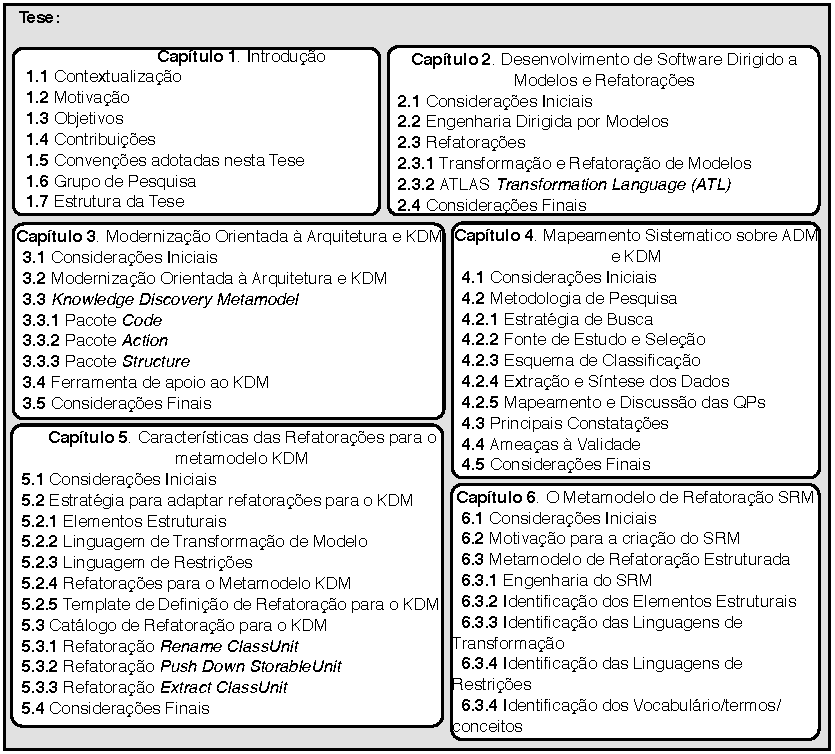
\includegraphics[scale=0.9]{images/PhD_Structure_Figure}
	%\fautor
%\end{figure}